\chapter{Arhitektura i dizajn sustava}
		
	Arhitektura se može podijeliti na tri podsustava: 
	\begin{itemize}
		\item Web poslužitelj 
		\item Web aplikacija 
		\item Baza podataka 
	\end{itemize}
	Web preglednik je program koji korisniku omogućuje pregled web stranica i multimedijalnih sadržaja vezanih uz njih. Svaki internetski preglednik je prevoditelj. Dakle, stranica je pisana u kodu koji preglednik nakon toga interpretira kako nešto svakome razumljivo. Korisnik putem web preglednika šalje zahtjev web poslužitelju. 
	
	Web poslužitelj osnova je rada web aplikacije. Njegova primarna zadaća je komunikacija klijenta s aplikacijom. Komunikacija se odvija preko HTTP (engl. Hyper Text Transfer Protocol) protokola, što je protokol u prijenosu informacija na webu. Poslužitelj je onaj koji pokreće web aplikaciju te joj prosljeđuje zahtjev. 
	
	Korisnik koristi web aplikaciju za obrađivanje željenih zahtjeva. Web aplikacija obrađuje zahtjev te ovisno o zahtjevu, pristupa bazi podataka nakon čega preko poslužitelja vraća korisniku odgovor u obliku HTML dokumenta vidljivog u web pregledniku. 
	
	Programski jezik kojeg smo odabrali za izradu naše web aplikacije je ???. Odabrano razvojno okruženje je ???. Arhitektura sustava temeljiti će se na MVC (Model-View-Controller) konceptu. 
	
	Karakteristika MVC koncepta je nezavisan razvoj pojedinih dijelova aplikacije što za posljedicu ima jednostavnije ispitivanje kao i jednostavnije razvijanje i dodavanje novih svojstava u sustav. \\
	
	MVC koncept sastoji se od: 
	\begin{itemize}
		\item Model - Središnja komponenta sustava. Predstavlja dinamičke strukture podataka, neovisne o korisničkom sučelju. Izravno upravlja podacima, logikom i pravilima aplikacije. Također prima ulazne podatke od Controllera 
		\item View - Bilo kakav prikaz podataka, poput grafa. Mogući su različiti prikazi iste informacije poput grafičkog ili tabličnog prikaza podatak. 
		\item Controller – Prima ulaze i prilagođava ih za prosljeđivanje Model-u ili View-u. Upravlja korisničkim zahtjevima i na temelju njih izvodi daljnju interakciju s ostalim elementima sustava. 
	\end{itemize}
		

		

				
		\section{Baza podataka}
			
			\textbf{\textit{dio 1. revizije}}\\
			
		\textit{Potrebno je opisati koju vrstu i implementaciju baze podataka ste odabrali, glavne komponente od kojih se sastoji i slično.}
		
			\subsection{Opis tablica}
			

				\textit{Svaku tablicu je potrebno opisati po zadanom predlošku. Lijevo se nalazi točno ime varijable u bazi podataka, u sredini se nalazi tip podataka, a desno se nalazi opis varijable. Svjetlozelenom bojom označite primarni ključ. Svjetlo plavom označite strani ključ}
				
				\begin{longtabu} to \textwidth {|X[6, l]|X[6, l]|X[20, l]|}
					
					\hline \multicolumn{3}{|c|}{\textbf{Djelatnik}}	 \\[3pt] \hline
					\endfirsthead
					
					\hline \multicolumn{3}{|c|}{\textbf{Djelatnik}}	 \\[3pt] \hline
					\endhead
					
					\hline 
					\endlastfoot
					
					\cellcolor{LightGreen}idDjelatnik & INTEGER	& Identifikator djelatnika.	\\ \hline
					ime	& VARCHAR & Ime djelatnika.  	\\ \hline 
					prezime & VARCHAR & Prezime djelatnika.  \\ \hline 
					OIB & VARCHAR & Osobni identifikacijski broj.		\\ \hline
					email & VARCHAR & E-mail adresa.		\\ \hline
					korisnickoIme & VARCHAR	& Jedinstveno korisničko ime djelatnika.	\\ \hline
					lozinka & VARCHAR & Lozinka djelatnika.		\\ \hline   
					\cellcolor{LightBlue} idUloga & INTEGER & Identifikator uloge djelatnika. 	\\ \hline 
					
					
				\end{longtabu}

				\begin{longtabu} to \textwidth {|X[6, l]|X[6, l]|X[20, l]|}
					
					\hline \multicolumn{3}{|c|}{\textbf{Uloga}}	 \\[3pt] \hline
					\endfirsthead
					
					\hline \multicolumn{3}{|c|}{\textbf{Uloga}}	 \\[3pt] \hline
					\endhead
					
					\hline 
					\endlastfoot
					
					\cellcolor{LightGreen}idUloga & INTEGER	& Identifikator uloge.	\\ \hline
					naziv & VARCHAR & Naziv uloge (direktor, vođa tima, djelatnik).  	\\ \hline 					
					
				\end{longtabu}
			
				\begin{longtabu} to \textwidth {|X[6, l]|X[6, l]|X[20, l]|}
					
					\hline \multicolumn{3}{|c|}{\textbf{Grupa}}	 \\[3pt] \hline
					\endfirsthead
					
					\hline \multicolumn{3}{|c|}{\textbf{Grupa}}	 \\[3pt] \hline
					\endhead
					
					\hline 
					\endlastfoot
					
					\cellcolor{LightGreen}idGrupa & INTEGER	& Identifikator grupe.	\\ \hline
					naziv	& VARCHAR & Naziv grupe.  	\\ \hline    
					\cellcolor{LightBlue} idVoditelj & INTEGER & Identifikator voditelja grupe. 	\\ \hline 
					\cellcolor{LightBlue} idDjelatnost & INTEGER & Identifikator djelatnosti kojom se grupa bavi. 	\\ \hline 
					
				\end{longtabu}
			
				\begin{longtabu} to \textwidth {|X[6, l]|X[6, l]|X[20, l]|}
					
					\hline \multicolumn{3}{|c|}{\textbf{jeClan}}	 \\[3pt] \hline
					\endfirsthead
					
					\hline \multicolumn{3}{|c|}{\textbf{jeClan}}	 \\[3pt] \hline
					\endhead
					
					\hline 
					\endlastfoot
					
					\cellcolor{LightGreen}idDjelatnik & INTEGER	& Identifikator djelatnika.	\\ \hline
					\cellcolor{LightGreen}idGrupa & INTEGER	& Identifikator grupe.	\\ \hline
					
				\end{longtabu}
			
				\begin{longtabu} to \textwidth {|X[6, l]|X[6, l]|X[20, l]|}
					
					\hline \multicolumn{3}{|c|}{\textbf{Djelatnost}}	 \\[3pt] \hline
					\endfirsthead
					
					\hline \multicolumn{3}{|c|}{\textbf{Djelatnost}}	 \\[3pt] \hline
					\endhead
					
					\hline 
					\endlastfoot
					
					\cellcolor{LightGreen}idDjelatnost & INTEGER	& Identifikator djelatnosti.	\\ \hline
					naziv & VARCHAR	& Naziv djelatnosti.	\\ \hline
					opis & VARCHAR	& Opis djelatnosti.	\\ \hline
					
				\end{longtabu}
			
				\begin{longtabu} to \textwidth {|X[10, l]|X[6, l]|X[16, l]|}
					
					\hline \multicolumn{3}{|c|}{\textbf{Zadatak}}	 \\[3pt] \hline
					\endfirsthead
					
					\hline \multicolumn{3}{|c|}{\textbf{Zadatak}}	 \\[3pt] \hline
					\endhead
					
					\hline 
					\endlastfoot
					
					\cellcolor{LightGreen}idZadatak & INTEGER	& Identifikator zadatka.	\\ \hline
					naziv & VARCHAR	& Naziv zadatka.	\\ \hline
					opis & VARCHAR	& Tekstualni opis zadatka.	\\ \hline
					datumVrijemePocetka & TIMESTAMP	& Datum i vrijeme početka zadatka. Mora biti manje vrijednosti od polja datumVrijemeZavrsetka.	\\ \hline
					datumVrijemeZavrsetka & TIMESTAMP	& Datum i vrijeme završetka zadatka. Mora biti veće vrijednosti od polja datumVrijemePocetka.	\\ \hline
					procjenaBrojaSati & INTEGER	& Procjena broja radnih sati potrebnih za dovršetak zadatka. Procjenu određuje voditelj tima koji je zadao zadatak. Procjena može, ali ne mora odgovarati razlici između datumVrijemeZavrsetka i datumVrijemePocetka. \\ \hline
					\cellcolor{LightBlue}idDjelatnost & INTEGER	& Identifikator djelatnosti kojoj zadatak pripada.	\\ \hline
					\cellcolor{LightBlue}idLokacija & INTEGER	& Identifikator lokacije na kojoj se zadatak obavlja.	\\ \hline
					
				\end{longtabu}
			
				\begin{longtabu} to \textwidth {|X[6, l]|X[6, l]|X[20, l]|}
					
					\hline \multicolumn{3}{|c|}{\textbf{radiNa}}	 \\[3pt] \hline
					\endfirsthead
					
					\hline \multicolumn{3}{|c|}{\textbf{radiNa}}	 \\[3pt] \hline
					\endhead
					
					\hline 
					\endlastfoot
					
					\cellcolor{LightGreen}idDjelatnik & INTEGER	& Identifikator djelatnika koji radi na zadatku.	\\ \hline
					\cellcolor{LightGreen}idZadatak & INTEGER	& Identifikator zadatka na kojem djelatnik radi.	\\ \hline
					realizacija & SMALLINT & Postotak posla kojeg je djelatnik obavio na zadatku u odnosu na ukupan posao. Može biti u intervalu [0, 100]. Početna vrijednost je 0. \\ \hline
					
				\end{longtabu}
			
				\begin{longtabu} to \textwidth {|X[6, l]|X[6, l]|X[20, l]|}
					
					\hline \multicolumn{3}{|c|}{\textbf{Lokacija}}	 \\[3pt] \hline
					\endfirsthead
					
					\hline \multicolumn{3}{|c|}{\textbf{Lokacija}}	 \\[3pt] \hline
					\endhead
					
					\hline 
					\endlastfoot
					
					\cellcolor{LightGreen}idLokacija & INTEGER	& Identifikator lokacije.	\\ \hline
					adresa & VARCHAR & Adresa na kojoj se lokacija nalazi. \\ \hline
					mjesto & VARCHAR & Mjesto u kojem lokacija nalazi. \\ \hline
					lat & DOUBLE & Geografska širina lokacije. \\ \hline
					long & DOUBLE & Geografska dužina lokacije. \\ \hline
					
				\end{longtabu}
			
				\begin{longtabu} to \textwidth {|X[6, l]|X[6, l]|X[20, l]|}
					
					\hline \multicolumn{3}{|c|}{\textbf{UnosRadnihSati}}	 \\[3pt] \hline
					\endfirsthead
					
					\hline \multicolumn{3}{|c|}{\textbf{UnosRadnihSati}}	 \\[3pt] \hline
					\endhead
					
					\hline 
					\endlastfoot
					
					\cellcolor{LightGreen}idUnos & INTEGER	& Identifikator unosa.	\\ \hline
					datum & DATE & Datum unosa. \\ \hline
					brRadnihSati & SMALLINT & Broj radnih sati koje je djelatnik odradio na zadatku tog dana. \\ \hline
					\cellcolor{LightBlue}idDjelatnik & INTEGER & Identifikator djelatnika koji obavlja unos. \\ \hline
					\cellcolor{LightBlue}idZadatak & INTEGER & Identifikator zadatka na kojeg se unos odnosi. \\ \hline
					
				\end{longtabu}
						
			\subsection{Dijagram baze podataka}
				\textit{ U ovom potpoglavlju potrebno je umetnuti dijagram baze podataka. Primarni i strani ključevi moraju biti označeni, a tablice povezane. Bazu podataka je potrebno normalizirati. Podsjetite se kolegija "Baze podataka".}
				
				\begin{figure}
					\centering
					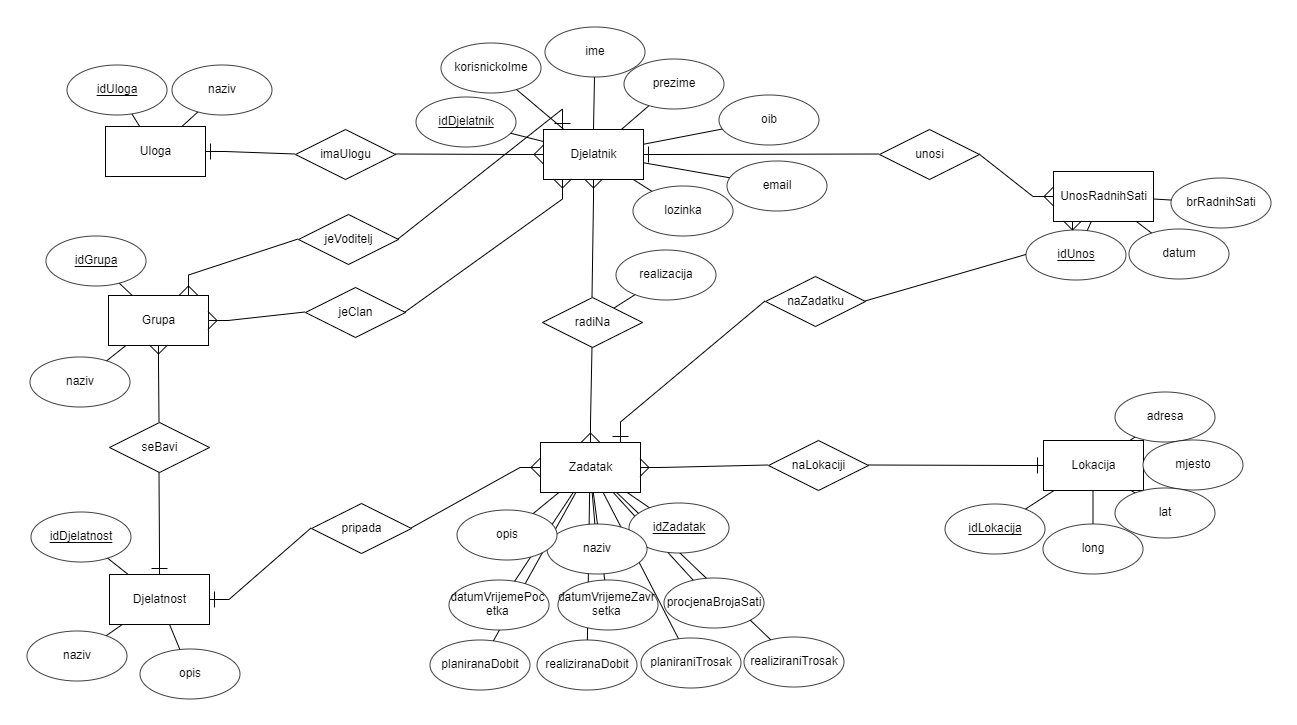
\includegraphics[width=\textwidth]{slike/ERdijagram.png}
					\caption{ER dijagram baze podataka}
				\end{figure}
			
				\begin{figure}
					\centering
					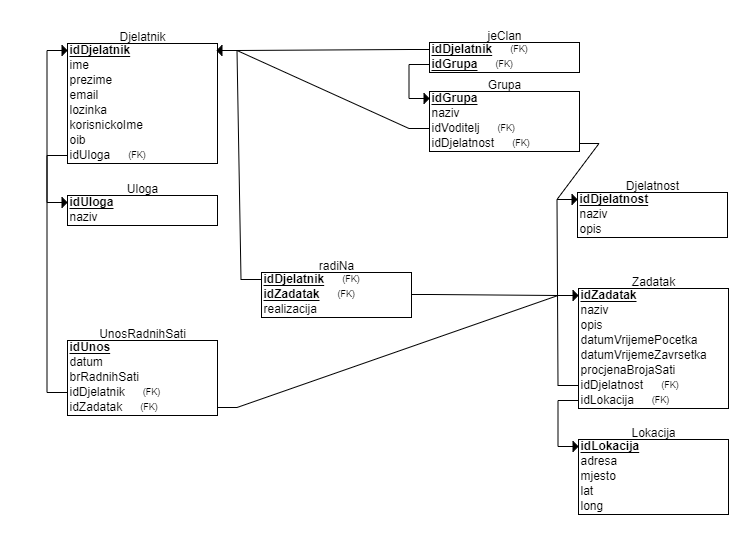
\includegraphics[width=\textwidth]{slike/RelDijagram.png}
					\caption{Relacijski dijagram baze podataka}
				\end{figure}		
			\eject
			
			
		\section{Dijagram razreda}
		
			\textit{Potrebno je priložiti dijagram razreda s pripadajućim opisom. Zbog preglednosti je moguće dijagram razlomiti na više njih, ali moraju biti grupirani prema sličnim razinama apstrakcije i srodnim funkcionalnostima.}\\
			
			\textbf{\textit{dio 1. revizije}}\\
			
			\textit{Prilikom prve predaje projekta, potrebno je priložiti potpuno razrađen dijagram razreda vezan uz \textbf{generičku funkcionalnost} sustava. Ostale funkcionalnosti trebaju biti idejno razrađene u dijagramu sa sljedećim komponentama: nazivi razreda, nazivi metoda i vrste pristupa metodama (npr. javni, zaštićeni), nazivi atributa razreda, veze i odnosi između razreda.}\\
			
			\textbf{\textit{dio 2. revizije}}\\			
			
			\textit{Prilikom druge predaje projekta dijagram razreda i opisi moraju odgovarati stvarnom stanju implementacije}
			
			
			
			\eject
		
		\section{Dijagram stanja}
			
			
			\textbf{\textit{dio 2. revizije}}\\
			
			\textit{Potrebno je priložiti dijagram stanja i opisati ga. Dovoljan je jedan dijagram stanja koji prikazuje \textbf{značajan dio funkcionalnosti} sustava. Na primjer, stanja korisničkog sučelja i tijek korištenja neke ključne funkcionalnosti jesu značajan dio sustava, a registracija i prijava nisu. }
			
			
			\eject 
		
		\section{Dijagram aktivnosti}
			
			\textbf{\textit{dio 2. revizije}}\\
			
			 \textit{Potrebno je priložiti dijagram aktivnosti s pripadajućim opisom. Dijagram aktivnosti treba prikazivati značajan dio sustava.}
			
			\eject
		\section{Dijagram komponenti}
		
			\textbf{\textit{dio 2. revizije}}\\
		
			 \textit{Potrebno je priložiti dijagram komponenti s pripadajućim opisom. Dijagram komponenti treba prikazivati strukturu cijele aplikacije.}